\documentclass{article}

\usepackage{calculator}
\usepackage{calculus}

\usepackage{fancyhdr}
\usepackage{extramarks}
\usepackage{amsmath}
\usepackage{amsthm}
\usepackage{amsfonts}
\usepackage{tikz}
\usepackage[plain]{algorithm}
\usepackage{algpseudocode}
\usepackage{tikz,pgfplots,multicol}
\usepackage[font=small,labelformat=empty]{caption}
\usetikzlibrary{automata,positioning,arrows,patterns}

%
% Basic Document Settings
%

\topmargin=-0.45in
\evensidemargin=0in
\oddsidemargin=0in
\textwidth=6.5in
\textheight=9.0in
\headsep=0.25in

\linespread{1.1}

\pagestyle{fancy}
\lhead{\hmwkAuthorName}
\chead{\hmwkClass\ (\hmwkClassInstructor\ \hmwkClassTime)}
\rhead{\hmwkTitle}
\lfoot{\lastxmark}
\cfoot{\thepage}

\renewcommand\headrulewidth{0.4pt}
\renewcommand\footrulewidth{0.4pt}

\setlength\parindent{0pt}

\setcounter{secnumdepth}{0}
\newcounter{partCounter}
\newcounter{homeworkProblemCounter}
\setcounter{homeworkProblemCounter}{1}
\nobreak\extramarks{Problem \arabic{homeworkProblemCounter}}{}\nobreak{}

%
% Homework Problem Environment
%
% This environment takes an optional argument. When given, it will adjust the
% problem counter. This is useful for when the problems given for your
% assignment aren't sequential. See the last 3 problems of this template for an
% example.
%
\newenvironment{homeworkProblem}[1][-1]{
    \ifnum#1>0
        \setcounter{homeworkProblemCounter}{#1}
    \fi
    \section{Problem \arabic{homeworkProblemCounter}}
    \setcounter{partCounter}{1}
    \enterProblemHeader{homeworkProblemCounter}
}{
    \exitProblemHeader{homeworkProblemCounter}
}

%
% Homework Details
%   - Title
%   - Due date
%   - Class
%   - Section/Time
%   - Instructor
%   - Author
%

\newcommand{\hmwkTitle}{HW \#7}
\newcommand{\hmwkDueDate}{March 2, 2017}
\newcommand{\hmwkClass}{MATH 1300}
\newcommand{\hmwkClassTime}{Section 005}
\newcommand{\hmwkClassInstructor}{Professor Braden Balentine}
\newcommand{\hmwkAuthorName}{\textbf{John Keller}}

%
% Title Page
%

\title{
    \vspace{2in}
    \textmd{\textbf{\hmwkClass:\ \hmwkTitle}}\\
    \normalsize\vspace{0.1in}\small{Due\ on\ \hmwkDueDate\ at 10:00am}\\
    \vspace{0.1in}\large{\textit{\hmwkClassInstructor\ \hmwkClassTime}}
    \vspace{3in}
}

\author{\hmwkAuthorName}
\date{}

\renewcommand{\part}[1]{\textbf{\large Part \Alph{partCounter}}\stepcounter{partCounter}\\}

%
% Various Helper Commands
%

% Useful for algorithms
\newcommand{\alg}[1]{\textsc{\bfseries \footnotesize #1}}

% For derivatives
\newcommand{\deriv}[1]{\frac{\mathrm{d}}{\mathrm{d}x} (#1)}

% For partial derivatives
\newcommand{\pderiv}[2]{\frac{\partial}{\partial #1} (#2)}

% Integral dx
\newcommand{\dx}{\mathrm{d}x}

% Alias for the Solution section header
\newcommand{\solution}{\textbf{\large Solution}}

% Probability commands: Expectation, Variance, Covariance, Bias
\newcommand{\E}{\mathrm{E}}
\newcommand{\Var}{\mathrm{Var}}
\newcommand{\Cov}{\mathrm{Cov}}
\newcommand{\Bias}{\mathrm{Bias}}


\usepackage{xcolor}
    \colorlet{Curve}{red!75!black}
    \colorlet{Tangent}{blue!75!black}
\usepackage{pgfplots}
    \pgfplotsset{compat=1.10}
    \usetikzlibrary{
        calc,
        intersections,
        math,
    }
    \makeatletter
        \def\parsenode[#1]#2\pgf@nil{%
            \tikzset{label node/.style={#1}}
            \def\nodetext{#2}
        }
        \tikzset{
            % define style for the points
            Point/.style={
                shape=circle,
                inner sep=0pt,
                minimum size=3pt,
            },
            add node at x/.style 2 args={
                name path global=plot line,
                /pgfplots/execute at end plot visualization/.append={
                        \begingroup
                        \@ifnextchar[{\parsenode}{\parsenode[]}#2\pgf@nil
                    \path [name path global = position line #1-1]
                        ({axis cs:#1,0}|-{rel axis cs:0,0}) --
                        ({axis cs:#1,0}|-{rel axis cs:0,1});
                    \path [xshift=1pt, name path global = position line #1-2]
                        ({axis cs:#1,0}|-{rel axis cs:0,0}) --
                        ({axis cs:#1,0}|-{rel axis cs:0,1});
                    \path [
                        name intersections={
                            of={plot line and position line #1-1},
                            name=left intersection
                        },
                        name intersections={
                            of={plot line and position line #1-2},
                            name=right intersection
                        },
                        label node/.append style={pos=1}
                    ] (left intersection-1) -- (right intersection-1)
                        node [label node]{\nodetext};
                    % ---------------------------------------------------------
                    % draw the tangent line from a bit right of the point on
                    % the curve to the intersection with the ordinate
                    % and draw the corresponding points
                    \draw [dashed] let
                        \p1=($ (left intersection-1) - (right intersection-1) $),
                        \p2=($ (left intersection-1)!sign(#1)*10mm!(right intersection-1) $),
                        %\p2=($ (left intersection+1) - (right intersection+1) $),
                        \p3=($ ({axis cs:0,0}) - (\p2) $),
                        \n1={\x3/\x1}	% slope of tangent line
                    in
                        (\p2) -- +($ {\n1}*(\x1,\y1) $)
	                        
%                        		node[right,node font=\scriptsize,gray] {$y=$\y1/\x1*sign(#1) $x+$}
%                            node [Point,fill=Tangent] (origin intersection) {}
                            node [Point,fill=Curve] at (left intersection-1) {}
                    ;
                    % ----------
                    % draw the horizontal line at the curve intersection point
                    % plus the label above/below the line
%                    \tikzmath{
%                        coordinate \c1;
%                        \c1=(left intersection-1) - (right intersection-1);
%                        \slope=\cy1/\cx1*sign(#1);
%                        \plusoffset = (#1+1);
%                    }
%                    \pgfmathsetmacro{\AboveBelow}{ \slope>0 ? "above" : "below" }
%                    \draw [dashed]
%                        ([xshift=sign(#1)*2.5mm] left intersection-1) --
%                        (left intersection-1) --
%                            node [\AboveBelow,node font=\scriptsize] {$y=\slope x+\plusoffset$}
%                        (left intersection-1 -| origin intersection) --
%                        +($ sign(#1)*(-2.5mm,0) $)
%                            coordinate [pos=0.5] (a)
%                    ;
%                    % draw the horizontal line at the ordinate intersection point
%                    \draw [dotted] (origin intersection)
%                        +($ sign(#1)*(-2.5mm,0) $) --
%                        (origin intersection);
%                    % draw vertical line left/right of the ordinate
%                    \pgfmathsetmacro{\LeftRight}{ #1<0 ? "right" : "left" }
%                    \draw [stealth-stealth] (origin intersection)
%                        +($ sign(#1)*(-1.25mm,0) $) -- (a)
%                            node [midway,\LeftRight,node font=\scriptsize] {$p$}
%                    ;
%                    % ---------------------------------------------------------
                        \endgroup
                },
            },
        }
    \makeatother
\makeatletter
\def\mathcolor#1#{\@mathcolor{#1}}
\def\@mathcolor#1#2#3{%
  \protect\leavevmode
  \begingroup
    \color#1{#2}#3%
  \endgroup
}
\makeatother


\begin{document}

\maketitle

\pagebreak

\section{Section 3.4}

\begin{enumerate}
\setcounter{enumi}{55}
	\item If $f$ is the function whose graph is shown, let $h(x)=f(f(x))$ and $g(x)=f(x^2)$. Use the graph of $f$ to estimate the value of each derivative.
		\begin{enumerate}
			\item $h'(2) = f'(1)\cdot -1 = -1 \cdot -1 = 1$
			\item $g'(2) = f'(2^2)\cdot 2(2) = 2\cdot 4 = 8$
		\end{enumerate}
		\begin{center}
			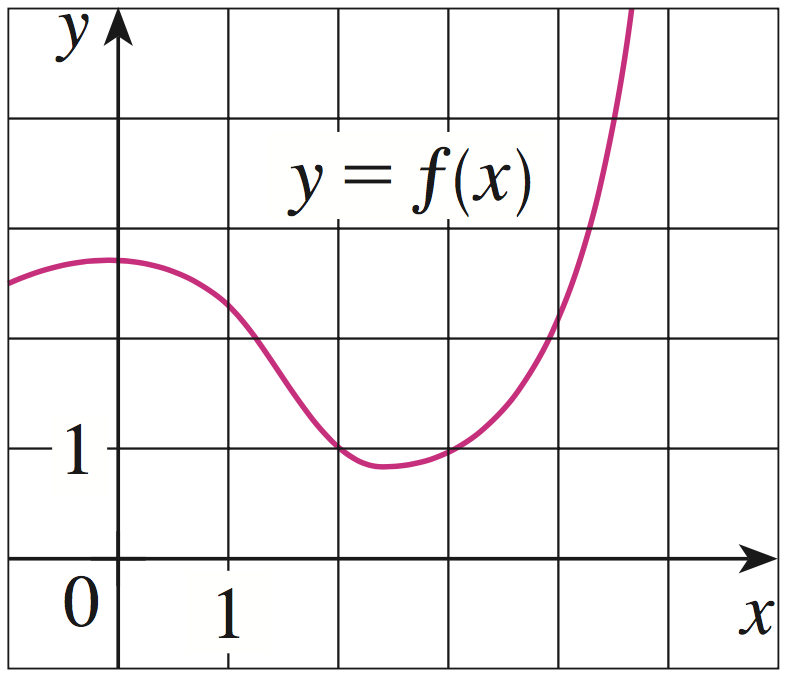
\includegraphics[width=3.5cm]{images/s34p56}
		\end{center}
\setcounter{enumi}{73}
	\item Under certain circimstances a rumor spreads according to the equation $$p(t)=\frac{1}{1+ae^{-kt}}$$ where $p(t)$ is the proportion of the population that knows the rumor at time $t$ and $a$ and $k$ are positive constants. [In section 7.5 we will see that this is a reasonable equation for $p(t)$.]
		\begin{enumerate}
			\item Find $\underset{t\rightarrow \infty}{\text{lim}}p(t)$.
				$$\begin{align}
					\underset{t\rightarrow \infty}{\text{lim}} \frac{1}{1+ae^{-kt}} &= \underset{t\rightarrow \infty}{\text{lim}}\frac{1}{1+\frac{a}{e^{kt}}}\\
					&= \frac{1}{1+0}\\
					&= 1
				\end{align}$$
			\item Find the rate of spread of the rumor.
				$$\begin{align}
					p'(t)&=\frac{(1+ae^{-kt})\cdot0 - 1\cdot(0+ae^{-kt}(-k)}{(1+ae^{-kt})^2}\\
					&= \frac{-(-ake^{-kt}}{(1+ae^{-kt})^2}\\
					&=\frac{ake^{-kt}}{(1+ae^{-kt})^2}
				\end{align}$$
			\item Graph $p$ for the case $a=10$, $k=0.5$ with $t$ measured in hours. Use the graph to estimate how long it will take for 80\% of the population to hear the rumor.
				\begin{center}
		\pgfplotsset{width=8cm,height=5cm}
%		\pgfplotsset{xmin=-10,xmax=10,ymin=-4,ymax=6,soldot/.style={color=blue,only marks,mark=*}
			\begin{tikzpicture}
			\begin{axis}[ymax=1,xlabel=$t$, ylabel=$p$,axis lines=middle,minor y tick num=0,minor x tick num=0,tick style={black},grid style={solid, gray!20}]
				\addplot[domain=0:10] {1/(1+10*exp(-0.5*x))};
				\addplot+[only marks,mark=*,mark options={fill=gray,scale=0.7},text mark as node=false,gray] coordinates {(7.4,0.8)};
			\end{axis}
		\end{tikzpicture}
				\end{center}
				Using the graph, it appears the rumor will take 7.4 hours to spread to 80\% of the population.
		\end{enumerate}
\end{enumerate}

\section{Section 3.5}
\begin{enumerate}
\setcounter{enumi}{34}
	\item If $xy+e^y = e$, find the value of $y''$ at the point where $x=0$.\newline
	$$\begin{align}
		xy + e^y &= e \\
0y + e^y &= e \\
e^y &= e \\
y + xy' + y'e^y &= 0 \\
1 + 0y' + y'e^1 &= 0 \\
1 + y'e &= 0 \\
y' &= \frac{-1}{e} \\
2y' + (x + e^y)y'' + (y')²e^y &= 0 \\
2(\frac{-1}{e} ) + (0 + e^1)y'' + (-1/e)^2e^1 &= 0 \\
-\frac{1}{e} + ey'' &= 0 \\
y'' &= \frac{1}{e^2}\\
	\end{align}$$
\setcounter{enumi}{43}
	\item The two curves are \textbf{orthogonal} if their tangent lines are perpendicular at each point of intersection. Show that the given families of curves are \textbg{orthogonal trajectories} of each other, that is, every curve in one family is orthogonal to every curve in the other family. Sketch both families of curves on the same axis. $$y=ax^3, \qquad x^2 + 3y^2=b$$
		$$\begin{align}
			\frac{dy}{dx}&= 3(ax)^2 \\ 
			2x+6y\frac{dy}{dx} &= b\frac{dy}{dx} \\
			6y\frac{dy}{dx}-b\frac{dy}{dx} &= -2x \\
			\frac{dy}{dx}(6y-b) &= -2x \\
			\frac{dy}{dx} &= 2x \\
			3(ax)^2 &= 2x
		\end{align}$$
\end{enumerate}
\pagebreak
\section{Section 4.1}
\begin{enumerate}
\setcounter{enumi}{9}
	\item A particle moves along the curve $y=\sqrt{1+x^3}$. As it reaches the point $(2,3)$, the $y$-coordinate is increasing at a rate of 4 cm/s. How fast is the $x$-coordinate of the point changing at that instant?\newline
	$$\begin{align}
		\frac{dy}{dx} &= 4\\
		y &= \frac{1}{2}(1+x^3)^{-\frac{1}{2}} (3x^2)\\
		3\frac{dx}{dx} &= \frac{1}{2}(1+2^3\frac{dy}{dx})^{-\frac{1}{2}} (3(2)^2\frac{dy}{dx})\\
		3 &= \frac{1}{2}(1+2^3\frac{dy}{dx})^{-\frac{1}{2}} (3(2)^2\frac{dy}{dx})\\
		3 &= \frac{1}{2}(1+2^3\frac{dy}{dx})^{-\frac{1}{2}} (3(2)^2\frac{dy}{dx})\\
		\frac{dy}{dx} ^= 1+\frac{\sqrt{5}}{2} \approx \boxed{2.1}
	\end{align}$$
\setcounter{enumi}{13}
	\item A street light is mounted on top of a 15-ft-tall pole. A man 6 ft tall walks away from the pole with a speed of 5 ft/s along a straight path. How fast is the top of his shadow moving when he is 40 ft from the pole?
		\begin{enumerate}
			\item What quantities are given in the problem?
				\begin{itemize}
					\item $\frac{dx}{dt}=5$ ft/s
					\item $h=15$ ft
					\item $h_2=6$ ft
					\item $b=40$ ft
				\end{itemize}
			\item What is the unknown?
				\begin{itemize}
					\item $y$
				\end{itemize}
			\item Draw a picture of the situation for any time $t$.
					\begin{center}
			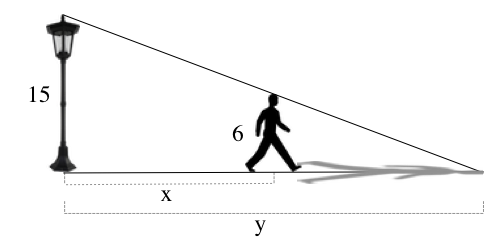
\includegraphics[width=6cm]{images/41pr14}
		\end{center}
			\item Write an equation that relates the quantities
				$$\frac{15}{y}=\frac{6}{y-x} \qquad \text{or} \qquad 9y=15x$$
			\item Finish solving the problem.
				$$\begin{align}
					9\frac{dy}{dt}&=15\frac{dx}{dt}\\
					9\frac{dy}{dt}&= 15(5)\\
					\frac{dy}{dt}&= \frac{25}{3} \text{ ft/s}
				\end{align}$$
		\end{enumerate}
\setcounter{enumi}{25}
	\item Water is leaking out of an inverted conical tank at a rate of 10,000 $\text{cm}^3$/min at the same time that water is being pumped into the tank at a constant rate. The tank has height 6 m and the diameter at the top is 4 m. If the water level is rising at a rate of 20 cm/min when the height of the water is 2 m, dins the rate at which water is being pumped into the tank. \newline
	\begin{itemize}
		\item $\frac{dV}{dt}=-10,000 \text{ cm}^3\text{/min}$
		\item $\frac{dh}{ht}= 200 \text{ cm}$
		\item $r=400$ cm
		\item $h=600$ cm
	\end{itemize}
	$$\begin{align}
		V&= \frac{1}{3}\pi\Big(\frac{1}{2}h\Big)^2h \\
		V&= \frac{1}{3}\pi \frac{1}{4}h^2 h \\
		\frac{dV}{dt} &= \frac{1}{3}\pi \frac{3}{4}\cdot 200^2 \cdot 20\\
		\frac{dV}{dt} &= \frac{3}{12}\pi 40,000(20)\\
		\frac{dV}{dt} &= \frac{1}{4}\pi 800,000\\
		\frac{dV}{dt} &= \boxed{200,000\pi - 10,000}
	\end{align}$$
\setcounter{enumi}{43}
	\item The minute hand on a watch is 8 mm long and the hour hand is 4 mm long. How fast is the distance between the hands changing at one o'clock?\newline
	\begin{itemize}
		\item Law of Cosines: $c^2=a^2+b^2-2ab \cos(C)$
	\end{itemize}
	$$\begin{align}
		c^2 &= 8^2 + 4^2 - 2(4)(8)\cos(C)\\
		c^2 &= 80-64 \cos(C)\\
		c^2 &= 80-64 \cos\Big(\frac{\pi	}{6}\Big) \\
		c^2 &= 80-64 \cdot \frac{\sqrt3}{2}\\
		c^2 &= 80-32\sqrt{3}\\
		c &= \sqrt{80-32\sqrt{3}}\\
		2c\frac{dc}{dt} &= 64 \sin(C) \frac{dC}{dt}\\
		2(\sqrt{80-32\sqrt{3}})\frac{dc}{dt} &= 64 \sin(\frac{\pi}{6}) (-\frac{11\pi}{6})\\
		2(\sqrt{80-32\sqrt{3}})\frac{dc}{dt} &= 64 \frac{1}{2} (-\frac{11\pi}{6})\\
		\sqrt{80-32\sqrt{3}}\frac{dc}{dt} &= -\frac{88\pi}{3}\\
		\frac{dc}{dt} &= -\frac{88\pi}{3\sqrt{80-32\sqrt{3}}} \approx 18 \text{ mm/hr}
	\end{align}$$
\end{enumerate}

\end{document}